\documentclass[20pt, a0paper, portrait]{tikzposter}

  \usepackage[utf8]{inputenc}
  \usepackage[T1]{fontenc}
  \usepackage{textcomp}
  \usepackage{arev}
  \usepackage{arevmath}
  \usepackage{arevtext}
  \usepackage{graphicx}
  \usepackage{wrapfig}
  \usepackage{microtype}
  \usepackage{booktabs}
  
  % Bibliography
  \usepackage[backend=biber,
  bibencoding=utf8,
  bibstyle=numeric-comp,
  %style=verbose, %verbose-ibid,
  url=true, % include url in reference
  doi=true, % include doi in reference
  sorting=none, % sorting of citations
  %autocite=superscript, % autocite becomes superscript
  maxcitenames=1, % Max names displayed when citing in text
  maxbibnames=10, % Max number of names displayed in the bibliography
  giveninits=true % Use initials
  ]{biblatex}
  \addbibresource{citations.bib}
  \renewcommand*{\bibfont}{\footnotesize}
  
  \renewcommand*\familydefault{\sfdefault}
  
  \title{Spur \& Helical Gear Guidelines}
  \author{Engineering Design \& Manufacture Group}
  \date{\today}
  \institute{University of Bath, UK}
  
  \usetheme{Default}
  \usecolorstyle[colorPalette=GreenGrayViolet]{Default}
  \useblockstyle{Default}
  \usetitlestyle{Filled}
    
  \begin{document}
  
  \maketitle
  
  \begin{columns}
    \column{0.5}
      \block[]{Introduction}{
        Two gears in mesh are called a gear pair. Normally gears mesh externally but sometimes the mesh may be internal, that is, one of the gears has the teeth cut internally. The smaller gear of a pair is called the pinion whereas the larger is called the wheel. In a pair of gears, the gear transmitting input torque and power is called the driver whereas the gear transmitting output torque and power is known as the driven. Normally in mechanical power transmission, the driver is the pinion so the wheel rotates at a slower speed than the pinion, that is, there is a reduction in speed through the gear pair. (You might like to discuss the reason why this is so).

        Usually gears are cylindrical but other forms are possible of which the most common is the rack and pinion. Here the wheel is flat (of infinite diameter) and is known as a rack.

        When more than two gears are in continuous mesh, this is known as a gear train. There are several types of gear train used in mechanical power transmission, including simple, compound and planetary. These are illustrated in Figure \ref{fig-1}.

        \begin{tikzfigure}[Gear Trains]\label{fig-1}
          \center
          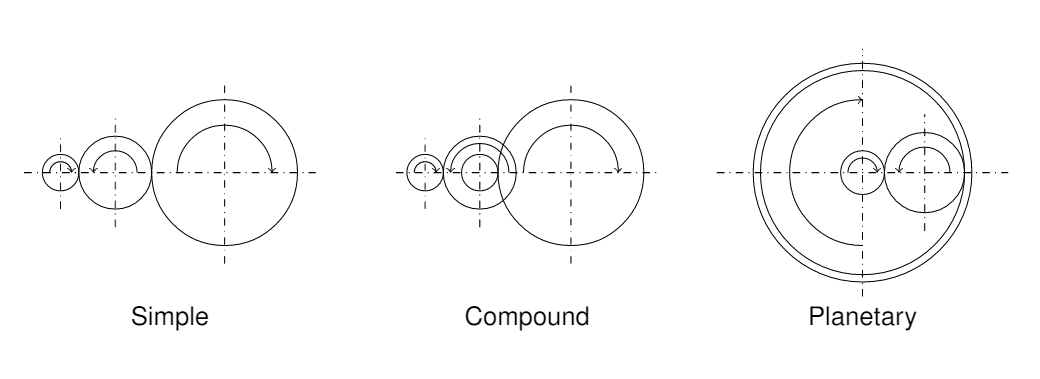
\includegraphics[width=0.3\textwidth]{figures/gear-trains.png}
        \end{tikzfigure}
      }
      \block[]{Velocity Ratio (VR)}{
        For all gears other than the worm and wheel, the velocity ratio of a gear pair is the ratio of the number of teeth in each gear. For example, if a 20 tooth pinion meshes with a 40 tooth wheel, the velocity ratio is:

        \begin{equation}
          \text{VR} = \frac{40}{20} = 2
        \end{equation}

        In the case of a compound gear train, the overall velocity ratio is the multiplication of the velocity ratio of each gear pair. If in the above example, the wheel had a 20 tooth pinion attached to it, that meshed with a 60 tooth wheel, the overall velocity ratio is:

        \begin{equation}
          \text{VR} = \frac{40}{20} \times \frac{60}{20} = 2 \times 3 = 6
        \end{equation}
      }
      \block[Number of Teeth]{}{
        It is impractical to have gears with too few teeth (just try and draw a gear with say 3 teeth). To get a reasonable tooth profile without undercutting and with a smooth transfer of power from pinion to wheel, a rule-of-thumb is that spur gears should have at least 17 teeth on the pinion and helical gears (\ang{20} helix angle) should have at least 14 teeth on the pinion.

        For maximum life with meshing gears it is desirable to distribute the wear uniformly amongst all teeth, that is not to have the same teeth in mesh for every revolution of the wheel. The best situation possible is that the same teeth mesh together again only after the pinion revolutions equals the number of teeth in the wheel. This is also known as having all the teeth hunting. For example if there are 40 teeth in the wheel, the best possible situation is that re-meshing of the same teeth occurs only after the pinion has made 40 revolutions. The condition for this is that the velocity ratio cannot be reduced to a simpler ratio, that is, there is no common factor between the number of teeth in the pinion and the number of teeth in the gear.

        Some possible combinations are given in Table \ref{tbl-1}.

        \begin{tikzfigure}[Pinion and wheel combinations]
          \label{tbl-1}
          \center
          \begin{tabular}{p{0.1\textwidth} p{0.1\textwidth} p{0.1\textwidth}}
            \toprule
            \textbf{Teeth in Pinion} & \textbf{Teeth in Wheel} & \textbf{Revolutions of the pinion when cycle repeats} \\
            \midrule
            18 & 38 & 19 \\
            19 & 38 & 2 \\
            20 & 38 & 19 \\
            21 & 38 & 38 \\
            18 & 40 & 20 \\
            19 & 40 & 20 \\
            20 & 40 & 2 \\
            21 & 40 & 40 \\
            \bottomrule
          \end{tabular}
        \end{tikzfigure}

        It can be seen therefore, that there can be a huge difference in the way wear will be distributed for approximately the same velocity ratio. However, in practice, exact velocity ratios are often needed (for example, for a camshaft) and in such cases, hunting teeth cannot be provided.
      }
    \column{0.5}
      \block[]{Gear Parameters}{
        Consider two gears in mesh as shown in Figure \ref{fig-3}:

        \begin{tikzfigure}[Meshing gears]\label{fig-3}
          \center
          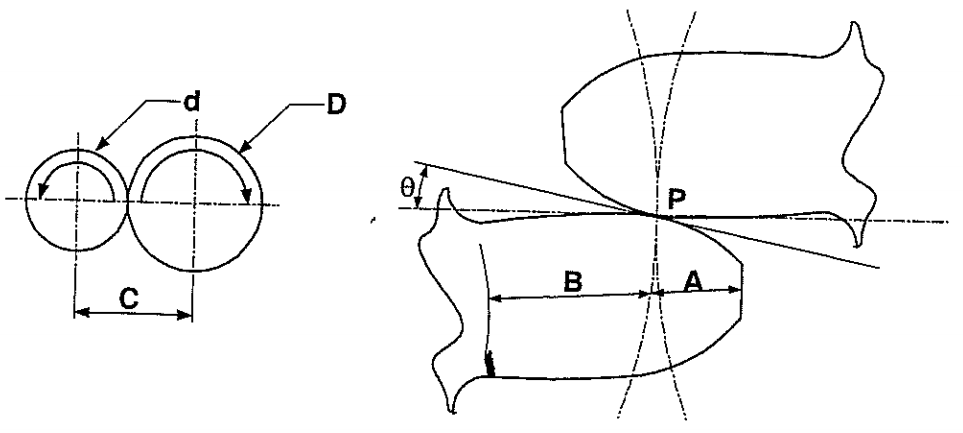
\includegraphics[width=0.2\textwidth]{figures/meshing-gears.png}
        \end{tikzfigure}

        If the pinion has $n$ teeth and $\text{PCD}=d$, and the wheel has $N$ teeth and $\text{PCD}=D$ then:

        \begin{equation}
          \text{VR} = \frac{N}{n} = \frac{D}{d}
        \end{equation}

        The nominal centre distance $C$ is:

        \begin{equation}
          C = 0.5(d+D)
        \end{equation}

        This is known as the nominal centre distance because the actual centre distance is usually somewhat greater than this.

        The height of a tooth above the PCD line is known as the addendum (A). The height of a tooth below the PCD line is known as the dedendum (B).

        The angle made by the tangent to the gears at the point of contact is called the pressure angle ($\theta$). This angle is usually \ang{20} and should be assumed so unless otherwise stated.

        The point of contact is called the pitch point (P). In order to obtain a constant velocity ratio the pitch point should not move as the gears move into and out of mesh. If the pitch point did move in and out with each mesh, then this would cause acceleration/deceleration with each mesh. If the gears are rotating at relatively high speeds this would cause high acceleration/deceleration with high inertia forces and accelerated wear.

        The pitch point remains fixed when the gears are cut with an involute profile. The involute profile can best be demonstrated by unwinding a thin cord from around a cylinder as shown in Figure~\ref{fig-4}.

        \begin{tikzfigure}[Involute profile]\label{fig-4}
          \center
          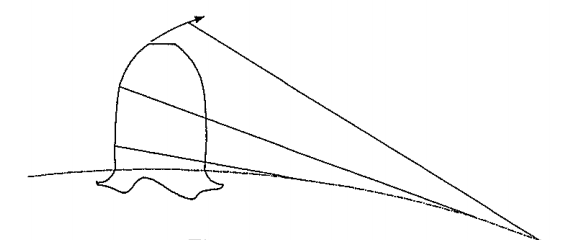
\includegraphics[width=0.2\textwidth]{figures/fig4.png}
        \end{tikzfigure}

        \textbf{Rack \& Pinion} In the case of a rack and pinion, the mating profile to the involute on the pinion is a straight sided rack as illustrated in Figure \ref{fig-5}. The angle of the rack is the pressure angle as previously defined

        \begin{tikzfigure}[Rack profile]\label{fig-5}
          \center
          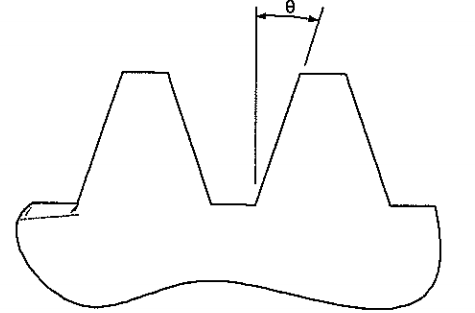
\includegraphics[width=0.2\textwidth]{figures/fig5.png}
        \end{tikzfigure}

        \textbf{Clearance} To minimise friction, the teeth should contact only along the front face of the driver and the back face of the driven. There should be both circumferential and radial clearance as shown in Figure~\ref{fig-6}.

        \begin{tikzfigure}[Clearance]\label{fig-6}
          \center
          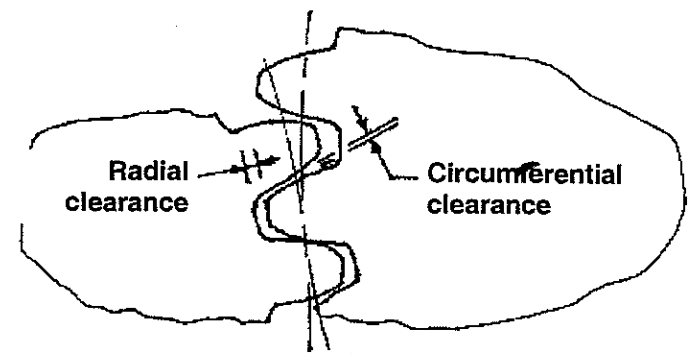
\includegraphics[width=0.2\textwidth]{figures/fig6.png}
        \end{tikzfigure}

        Radial clearance (or bottom clearance) is obtained by making the dedendum greater than the addendum. Usually $\text{B}=1.25\text{A}$. Circumferential clearance is usually very small when the gears are new because wear automatically increases it. It can be obtained by making the centre distance slightly larger than the nominal centre distance. Circumferential clearance causes \textbf{backlash} and can be measured by holding one gear fixed and moving the other gear back and forth relative to it.

      }
      \block[]{References}{
        \printbibliography[heading=none]{}
      }
  \end{columns}
  
  \end{document}